\subsection{Simulation Methodology}
\textit{xcopterCalc}\cite{ecalc}, a free tool provided by \textit{eCalc}, is utilized to reliably simulate multirotor parameters. This tool is widely used throughout the multirotor design community --- \textit{eCalc} is partnered with several prominent multirotor manufacturers (such as LeoMotion, DualSky, and more)\cite{ecalcpartner}. Through the use of \textit{xcopterCalc}, differing model parameters (such as battery size, payload weight, and propeller selection) can be tweaked in order to obtain a reasonable estimate for the multirotor's actual flight performance. 

It is important to stress that the figures extracted from \textit{xcopterCalc} are \textit{only estimates}. While the tool often makes conservative estimates (for example, a 3S 5000 mAh LiPo was measured to weigh 360 g while modeled to weigh 420 g in \textit{xcopterCalc}), it also neglects several real-world non-idealities. Examples of ignored non-idealities include high-frequency disturbances to control systems and the electric power consumption of the flight control unit and its sensors. 

There also exists limitations regarding the selection of motor and propeller models. The simulation calculates the driving performance of the motors (i.e. their power consumption and mechanical power output) through the use of a database containing performance characteristics submitted by parts manufacturers. The motors and propellers ultimately purchased for the final implementation are not listed within this database, and thus similar (near-identical) models had to be substituted in for use within the simulation.

\subsection{Design Verification}
To verify the performance of the final part selection (as detailed in the \textit{Design Document}), two simulations were performed with differing model weights -- 1200g and 600g. The model weight denotes the weight of the system excluding the powertrain. In other words, the model weight denotes the combined weight of the drone frame, flight accessories, and computation platform (including the computation platform battery). The fixed design and environmental parameters, used across both tests, are listed in Table \ref{env_param}.

\begin{table}[H]
\label{env_param}
\centering
\begin{tabular}{|l|l|}
\hline
Number of Rotors    & 4        \\ \hline
Frame Size          & 560 mm   \\ \hline
Controller Amperage & 30 A     \\ \hline
Field Elevation     & 100 m    \\ \hline
Air Temperature     & 25$^{\circ}$ C     \\ \hline
Pressure            & 1013 hPa \\ \hline
\end{tabular}
\caption{Fixed Design and Environmental Parameters}
\end{table}

Screenshots of the simulations, outlining all expected parameters, are included in each subsection below. A summary of the results is seen in Table \ref{summary}.

\begin{table}[]
\centering
\begin{tabular}{|l|l|l|}
\hline
\textbf{Model Weight (g)}              & \textbf{1200}       & \textbf{600}        \\ \hline
Battery Size                  & 3S 5000mAh & 3S 5000mAh \\ \hline
Hover Flight Time (min)       & 9.9        & 16         \\ \hline
Thrust:Weight Ratio           & 1.7        & 2.3        \\ \hline
Thrust (g/W)                  & 7.21       & 8.43       \\ \hline
Maximum Power Consumption (W) & 171.2      & 171.2      \\ \hline
\end{tabular}
\caption{Simulated Performance of Final Part Selection}
\label{summary}
\end{table}

\subsubsection{1200 g Model Weight Simulation}

\begin{figure}[H]
\centering
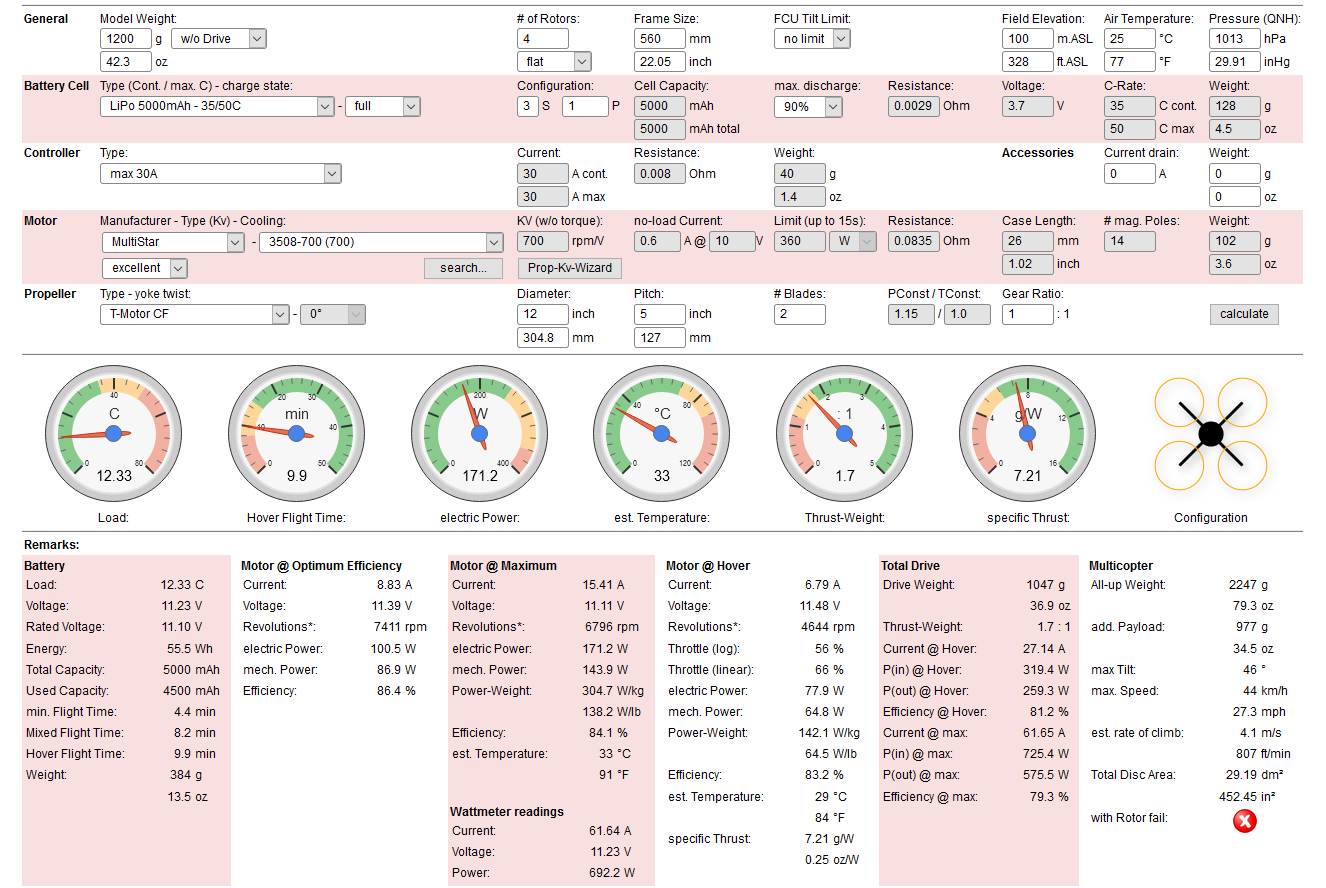
\includegraphics[width=16.5cm]{img/1200g_sim.png}
\caption{\textit{xcopterCalc} Output for 1200 g Model Weight}
\end{figure} 

\begin{figure}[H]
\centering
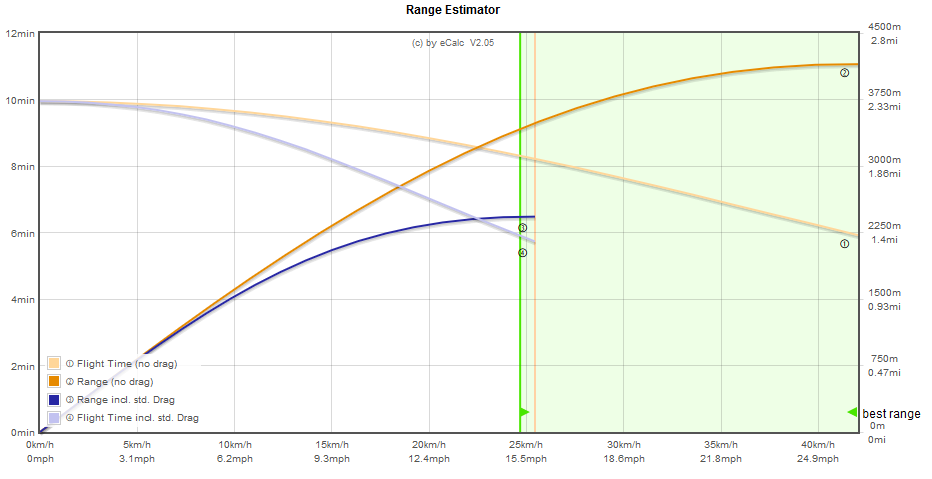
\includegraphics[width=16.5cm]{img/1200g_range.png}
\caption{Expected Range for 1200 g Model Weight}
\end{figure} 

\begin{figure}[H]
\centering
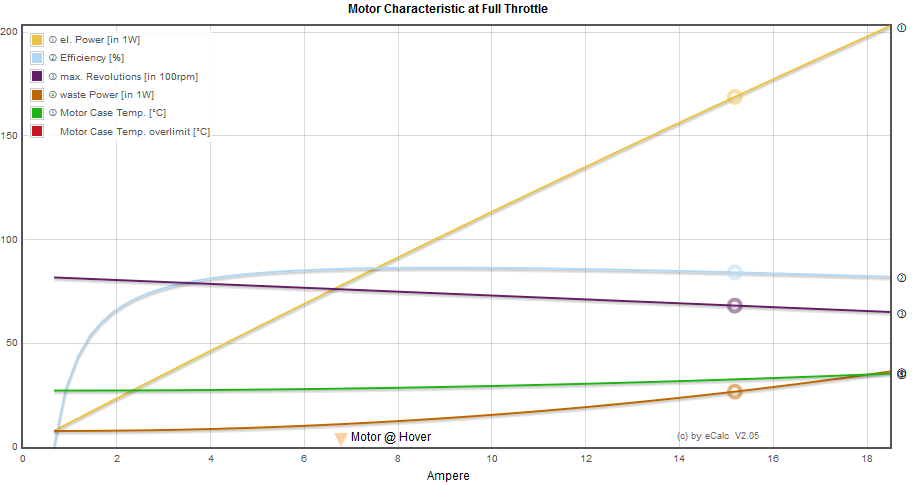
\includegraphics[width=16.5cm]{img/1200g_motor.png}
\caption{Motor Characteristics for 1200 g Model Weight}
\end{figure} 

\subsubsection{600 g Model Weight Simulation}

\begin{figure}[H]
\centering
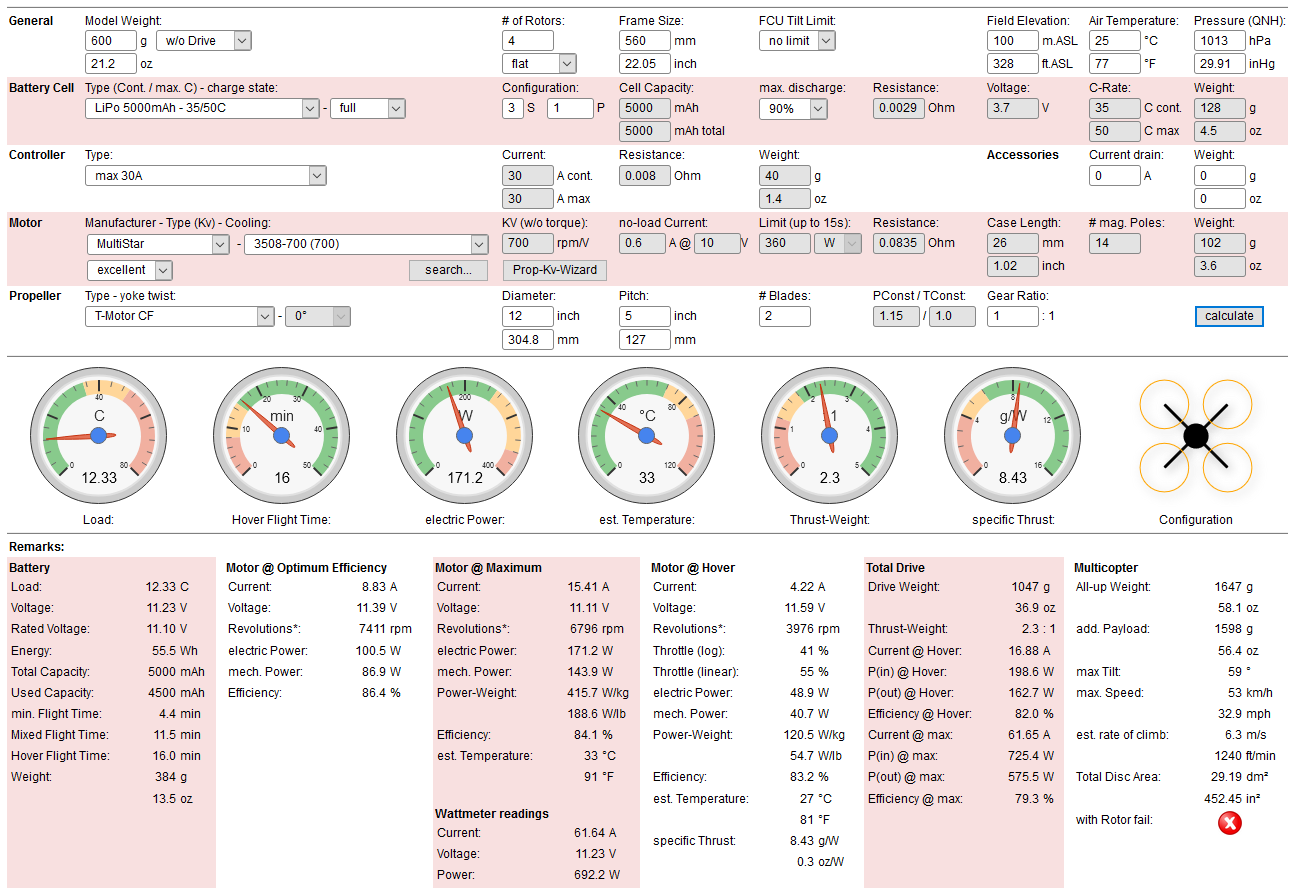
\includegraphics[width=16.5cm]{img/600g_sim.png}
\caption{\textit{xcopterCalc} Output for 600 g Model Weight}
\end{figure} 

\begin{figure}[H]
\centering
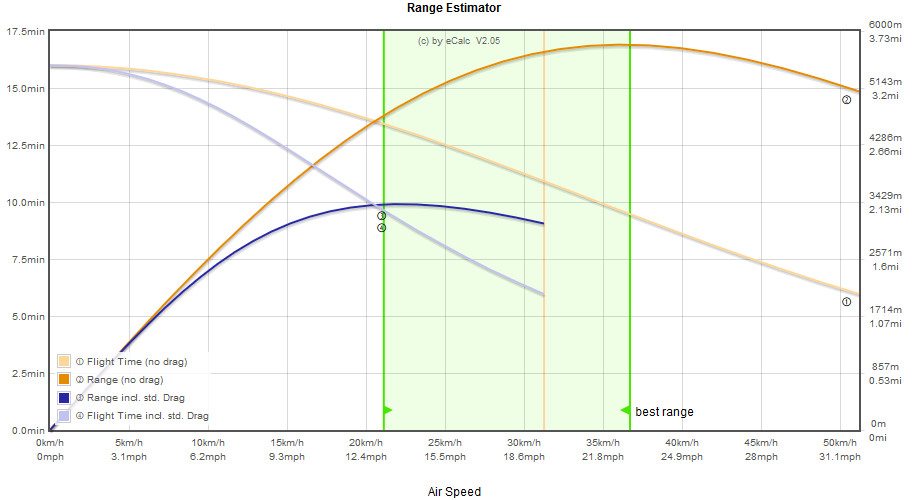
\includegraphics[width=16.5cm]{img/600g_range.png}
\caption{Expected Range for 600 g Model Weight}
\end{figure} 

\begin{figure}[H]
\centering
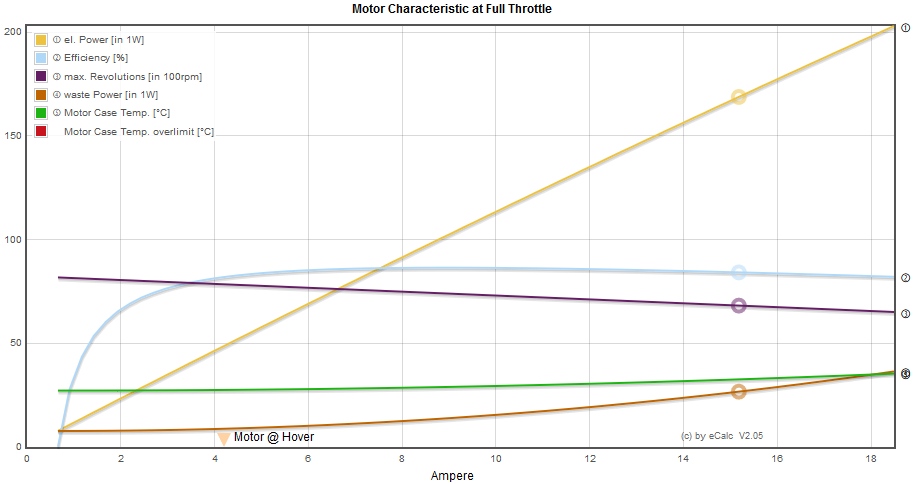
\includegraphics[width=16.5cm]{img/600g_motor.png}
\caption{Motor Characteristics for 600 g Model Weight}
\end{figure} 
\clearpage

\subsection{Payload Weight Variations}
As the client may wish to extend the functionality of the multirotor by adding or replacing components of the computing platform or multirotor, simulations have been performed to provide insight as to the impact of payload weight on flight performance. In particular, the following simulations measure maximum hover time across differing model weights, battery configurations (ex. 3S/4S), and battery capacities. All other (non-weight-related) parameters are kept constant across tests.

\begin{figure}[H]
\centering
\begin{subfigure}{.5\textwidth}
\begin{tikzpicture}
\pgfplotsset{compat=1.3}
\centering
\begin{axis}[
  xlabel=Total Model Weight (grams),
  ylabel=Hover Time (minutes),
  ylabel shift = -5 pt]
\addplot table [y=flightduration, x=weight]{plots/3S-5000.txt};
\addlegendentry{5 Ah}
\addplot table [y=flightduration, x=weight]{plots/3S-6000.txt};
\addlegendentry{6 Ah}
\addplot table [y=flightduration, x=weight]{plots/3S-10000.txt};
\addlegendentry{10 Ah}
\end{axis}
\end{tikzpicture}
\caption{Simulated Hover Times for 3S Batteries}
\end{subfigure}%
\begin{subfigure}{.5\textwidth}
\centering
\begin{tikzpicture}
\pgfplotsset{compat=1.3}
\begin{axis}[
  xlabel=Total Model Weight (grams),
  ylabel=Hover Time (minutes),
  ylabel shift = -5 pt]
\addplot table [y=flightduration, x=weight]{plots/4S-5000.txt};
\addlegendentry{5 Ah}
\addplot table [y=flightduration, x=weight]{plots/4S-6000.txt};
\addlegendentry{6 Ah}
\addplot table [y=flightduration, x=weight]{plots/4S-10000.txt};
\addlegendentry{10 Ah}
\end{axis}
\end{tikzpicture}
\caption{Simulated Hover Times for 4S Batteries}
\end{subfigure}
\end{figure}
\subsection{Propulsion Performance Exploration}
\label{prop_explore}

In order to increase the effective range and flight duration of the multirotor, the client may wish to install higher-capacity batteries (or alter their configurations). The following simulations sweep potential battery capacities and outline their impact on hover time, mixed flight time, and weight capacities.

\begin{figure}[H]
\centering
\begin{subfigure}{.5\textwidth}
\begin{tikzpicture}[scale=0.95]
\pgfplotsset{compat=1.3}
\centering
\begin{axis}[
  xlabel=Battery Capacity (Ah),
  ylabel=Flight Duration (minutes),
  ylabel shift = -5 pt,
  legend pos=south east]
\addplot table [y=hover, x=capacity]{plots/3S-time.txt};
\addlegendentry{Hover Flight}
\addplot table [y=mixed, x=capacity]{plots/3S-time.txt};
\addlegendentry{Mixed Flight}
\end{axis}
\end{tikzpicture}
\caption{3S Batteries}
\end{subfigure}%
\begin{subfigure}{.5\textwidth}
\centering
\begin{tikzpicture}[scale=0.95]
\pgfplotsset{compat=1.3}
\centering
\begin{axis}[
  xlabel=Battery Capacity (Ah),
  ylabel=Flight Duration (minutes),
  ylabel shift = -5 pt,
  legend pos=south east]
\addplot table [y=hover, x=capacity]{plots/4S-time.txt};
\addlegendentry{Hover Flight}
\addplot table [y=mixed, x=capacity]{plots/4S-time.txt};
\addlegendentry{Mixed Flight}
\end{axis}
\end{tikzpicture}
\caption{4S Batteries}
\end{subfigure}
\caption{Simulated Flight Times for Varying Battery Capacities}
\label{flighttime}
\end{figure}

\begin{figure}[H]
\centering
\begin{subfigure}{.5\textwidth}
\begin{tikzpicture}[scale=0.95]
\pgfplotsset{compat=1.3}
\centering
\begin{axis}[
  xlabel=Battery Capacity (Ah),
  ylabel=Weight (grams),
  legend style={at={(0.5,-0.2)},anchor=north},
  ylabel shift = -5 pt]
\addplot table [y=multirotor, x=capacity]{plots/3S-weight.txt};
\addlegendentry{Multirotor Weight}
\addplot table [y=payload, x=capacity]{plots/3S-weight.txt};
\addlegendentry{Payload Capacity}
\addplot table [y=total, x=capacity]{plots/3S-weight.txt};
\addlegendentry{Maximum Takeoff Weight}
\end{axis}
\end{tikzpicture}
\caption{3S Batteries}
\end{subfigure}%
\begin{subfigure}{.5\textwidth}
\centering
\begin{tikzpicture}[scale=0.95]
\pgfplotsset{compat=1.3}
\centering
\begin{axis}[
  xlabel=Battery Capacity (Ah),
  ylabel=Weight (grams),
  legend style={at={(0.5,-0.2)},anchor=north},
  ylabel shift = -5 pt]
\addplot table [y=multirotor, x=capacity]{plots/4S-weight.txt};
\addlegendentry{Multirotor Weight}
\addplot table [y=payload, x=capacity]{plots/4S-weight.txt};
\addlegendentry{Payload Capacity}
\addplot table [y=total, x=capacity]{plots/4S-weight.txt};
\addlegendentry{Maximum Takeoff Weight}
\end{axis}
\end{tikzpicture}
\caption{4S Batteries}
\end{subfigure}
\caption{Simulated Weights for Varying Battery Capacities}
\label{flightweight}
\end{figure}
As seen in Figure \ref{flighttime}, as battery capacity increases there is an asymptotic increase in both hover and mixed flight time. This non-linear behaviour stems from the increased weight demands of the higher capacity batteries -- a trend also evident in Figure \ref{flightweight} wherein higher capacity batteries take up a majority of the maximum take-off weight.
